\documentclass[twoside]{article}

\usepackage[a4paper, total={674pt, 426pt}, landscape]{geometry}
\usepackage{multicol}

\newcommand{\todo}[1]{\textcolor{red}{\textbf{TODO:} #1}}
\newcommand{\dyade}[1]{\overleftrightarrow{#1}}
\newenvironment{definition}[1]{\begin{tcolorbox}[title=Def.: #1, colback=white!,colframe=green!50!black]}{\end{tcolorbox}}

\titlespacing*{\section}{0pt}{.6\baselineskip}{.1\baselineskip}
\titlespacing*{\subsection}{0pt}{.6\baselineskip}{.1\baselineskip}
\titlespacing*{\subsubsection}{0pt}{.6\baselineskip}{.1\baselineskip}


%% This is the space for custom commands for your Formelsammlung
\newcommand{\FormelsammlungTitel}{Computational and Analytical Methods in Electromagnetics}
\newcommand{\FormelsammlungAutor}{Bogdan Stamenic}
\setcounter{tocdepth}{2} % Show only sections and subsection in table of contents

\begin{document}
	\title{\FormelsammlungTitel}
	\author{\FormelsammlungAutor}
	\date{\today}
	\begin{multicols*}{3}
%		\begin{minipage}{.4\paperheight}
			\maketitle
			\tableofcontents
%		\end{minipage}
		
\section{Fundamentals of Electromagnetic Fields}
\subsection{Maxwell's Equations}
Maxwell's Equations (integral form):
\begin{align*}
  \oint\limits_{C(A)} \vec{h}(\vec{r}, t)\cdot\mathrm{d}\vec{s}
  &= \iint\limits_{A}\left[ \vec{j}(\vec{r}, t) + \dfrac{\mathrm{d}\vec{d}(\vec{r}, t)}{\mathrm{d}t} \right]\cdot\mathrm{d}\vec{a}\\
  \oint\limits_{C(A)} \vec{e}(\vec{r}, t)\cdot\mathrm{d}\vec{s}
  &= -\iint\limits_{A}\left[ \vec{m}(\vec{r}, t) + \dfrac{\mathrm{d}\vec{b}(\vec{r}, t)}{\mathrm{d}t} \right]\cdot\mathrm{d}\vec{a}\\
  \oiint\limits_{A(V)}\vec{d}(\vec{r}, t)\cdot\mathrm{d}\vec{A} &= \iiint\limits_{V}\rho(\vec{r},t)\,\mathrm{d}v\\
  \oiint\limits_{A(V)}\vec{b}(\vec{r}, t)\cdot\mathrm{d}\vec{A} &= \iiint\limits_{V}\rho_{m}(\vec{r},t)\,\mathrm{d}v
\end{align*}

Maxwell's Equations (differential form):
\begin{align*}
&\nabla\times\vec{h}(\vec{r}, t) = \vec{j}(\vec{r},t) + \dfrac{\mathrm{d}\vec{d}(\vec{r},t)}{\mathrm{d}t}\\
&\nabla\times\vec{e}(\vec{r}, t) = -\dfrac{\mathrm{d}\vec{b}(\vec{r},t)}{\mathrm{d}t} -\vec{m}(\vec{r},t)\\
&\nabla\cdot\vec{d}(\vec{r},t) = \rho(\vec{r},t)\\
&\nabla\cdot\vec{b}(\vec{r},t) = \rho_{m}(\vec{r},t)
\end{align*}

Material Relations:
\begin{align*}
&\vec{d}(\vec{r},t) = \epsilon(\vec{r},t) * \vec{e}(\vec{r},t)\\
&\vec{j}(\vec{r},t) = \sigma(\vec{r},t) * \vec{e}(\vec{r},t) + \vec{j}_{\mathrm{exc}}(\vec{r},t)\\
&\vec{b}(\vec{r},t) = \mu(\vec{r},t) * \vec{h}(\vec{r},t)\\
&\vec{m}(\vec{r},t) = \vec{m}_{\mathrm{exc}}(\vec{r},t)\\
\end{align*}

Poisson Equation ($\partial_{t}\vec{e} = 0$, $\epsilon(\vec{r}) = \mathrm{const.}$):
\begin{equation*}
\nabla\cdot\left(\nabla\phi\right) = \Delta\phi = -\dfrac{\rho(\vec{r})}{\epsilon}
\end{equation*}

\subsection{Green's Theorems and Uniqueness of the Poisson Equation}
\todo{Add Green's theorems\\}
Solutions of $\Delta\phi(\vec{r}) = -\rho(\vec{r})/\epsilon$ are uniquely defined by specifying:
\begin{enumerate}
\item $\rho(\vec{r})$ and $\left.\phi(\vec{r})\right|_{\vec{r}\in F(V)}$
\item \textbf{or} $\rho(\vec{r})$ and $\left.\dfrac{\partial}{\partial n}\phi(\vec{r})\right|_{\vec{r}\in F(V)}$
\item \textbf{or} $\rho(\vec{r})$ and $\left.\phi(\vec{r})\right|_{\vec{r}\in F_{1}(V)}$, $\left.\dfrac{\partial}{\partial n}\phi(\vec{r})\right|_{\vec{r}\in F_{2}(V)}$\\
        with $F_{1}(V) \cup F_{2}(V) = F(V)$,\\
        $F_{1}(V) \cap F_{2}(V) = \emptyset$
\end{enumerate}

\subsection{Uniqueness of Time-Harmonic Electromagnetic Fields}
Unique solutions while assuming arbitrarily small losses, when:
\begin{enumerate}
\item Presetting $\vec{n}\times\vec{E}$ on boundary surface $A$
\item Presetting $\vec{n}\times\vec{H}$ on $A$
\item Presetting $\vec{n}\times\vec{E}$ on parts of $A$, presetting $\vec{n}\times\vec{H}$ on the remainder of $A$
\item In general, it is also possible to define $\vec{n}\times\vec{E}$ as a function of $\vec{n}\times\vec{H}$ or vice-versa
\end{enumerate}

\subsection{The Dirac Delta-Functional}
\begin{itemize}
  \item Motivated by volume charge density representation of a point charge:
      \begin{equation*}
        \iiint\limits_{V}\rho(\vec{r}, \vec{r_{P}})\mathrm{d}v =
        \begin{cases}
          Q_{P} \quad \text{for }\vec{r_{P}}\in V\\
          0 \quad \text{elsewhere}
        \end{cases}
      \end{equation*}
  \item Dirac delta defined via functional equation
        \begin{equation*}
\int\limits^{+\infty}_{-\infty}\delta(x)\varphi(x)\,\mathrm{d}x = \varphi(x)
        \end{equation*}
  \item A functional maps \textbf{a function onto a number}
        \begin{equation*}
\varphi(x) \mapsto \varphi(0)
        \end{equation*}
  \item A functional is linear, when
        \begin{align*}
&F\{\varphi_{1}+\varphi_{2}\} = F\{\varphi_{1}\} + F\{\varphi_{2}\}\\
&F\{k\varphi\} = kF\{\varphi\}
        \end{align*}
        \item Domain of functionals are \textit{function spaces}
        \item Function space is in general a set of functions and maps from a set $X$ onto a set $Y$
        \item In many cases, vector addition and scalar multiplication can be defined. Such function spaces are called \textit{vector spaces}.
        \item Properties of $\delta_{n}(x)$:
        \begin{align*}
          &\delta_{n}(ax) = \dfrac{1}{|a|} \delta(x)\\
          &\int\limits^{+\infty}_{-\infty}\delta^{(n)}\varphi(x)\,\mathrm{d}x = (-1)^{n}\varphi^{(n)}(0)\\
          &H^{\prime}(x) = \delta(x),\quad H(x) =
          \begin{cases}
            1 \quad x\geq0\\
            0 \quad \text{elsewhere}
          \end{cases}
        \end{align*}
\end{itemize}
\subsubsection{Multi-dimension $\delta$-distributions in different coordinate systems}
\begin{enumerate}
\item Cartesian coordinates $P=(x',y',z')$
        \begin{equation*}
          \mathrm{d}v = \mathrm{d}x\,\mathrm{d}y\,\mathrm{d}z
        \end{equation*}
        \begin{align*}
          \delta(\vec{r}-\vec{r}_{P}) = \delta(x-x')\delta(y-y')\delta(z-z')
        \end{align*}
\item Cylinder coordinates $P=(\rho',\varphi',z')$
        \begin{equation*}
          \mathrm{d}v = \rho\,\mathrm{d}\rho\,\mathrm{d}\varphi\,\mathrm{d}z
        \end{equation*}
        \begin{align*}
          &\delta(\vec{r}-\vec{r}_{P}) =\\
          &\begin{cases}
            \dfrac{1}{\rho}\delta(\rho-\rho')\delta(\varphi-\varphi')\delta(z-z'), \quad \rho'\neq0\\
            \dfrac{1}{\pi\rho}\delta(\rho)\delta(z-z'), \quad \rho'=0
          \end{cases}
        \end{align*}
\item Cylinder coordinates $P=(r',\vartheta',\varphi')$
        \begin{equation*}
          \mathrm{d}v = r^{2}\,\mathrm{d}r\,\sin(\vartheta)\,\mathrm{d}\,\vartheta\mathrm{d}\varphi
        \end{equation*}
        \begin{align*}
          &\delta(\vec{r}-\vec{r}_{P}) =\\
          &\begin{cases}
            \dfrac{1}{r^{2}\sin\vartheta}\delta(r-r')\delta(\vartheta-\vartheta')\delta(\varphi-\varphi'),r'\neq0\\
            \dfrac{1}{2\pi r^{2}}\delta(r), \quad r'=0
          \end{cases}
        \end{align*}
\end{enumerate}

		\section{Finite Difference and Integration Methods}

\subsection{Finite Difference Solution of Wave Problems in the Time Domain}
\begin{info}{Courant stability condition}
  In order for the FDTD-method to be stable, the so-called Courant-condition must be fulfilled:
  \begin{equation*}
    \Delta t \leq \left(c\sqrt{\dfrac{1}{(\Delta x)^{2}} + \dfrac{1}{(\Delta y)^{2}} + \dfrac{1}{(\Delta z)^{2}}}\,\right)^{-1},
  \end{equation*}
  where $\Delta t$, $\Delta x$, $\Delta y$, and $\Delta z$ are the discretization step sizes.
\end{info}

\subsection{Finite Integration Technique}
\begin{itemize}
        \item Mathematically identical to FD method
        \item Starting with the integral of Maxwell's Equations, \textit{replace the line and surface integrals} by discrete grid voltages $e_{x/y,i}$ and discrete grid fluxes $b_{z,j}$.
        \begin{align*}
          \oint\limits_{C(A)} \vec{e}(\vec{r}, t)\cdot\mathrm{d}\vec{s} = -\iint\limits_{A}\dfrac{\partial\vec{b}(\vec{r}, t)}{\partial t}\cdot\mathrm{d}\vec{a}\\
          \implies (\hat{e}_{x1} - \hat{e}_{x2}) + (\hat{e}_{y1} - \hat{e}_{y2}) = -\dot{\dhat{b_{z}}}
        \end{align*}
  \item The unknown grid voltages and grid fluxes are collected into column vectors and the discrete Maxwell equations can be written in the following matrix-vector form:
        \begin{align*}
          &\bs{C} \hat{\bs{e}} = -\dot{\dhat{\bs{b}}} & \text{(Faraday)}\\
          &\tilde{\bs{C}} \hat{\bs{h}} = \dot{\dhat{\bs{d}}} + \dhat{\bs{j}} & \text{(Ampère-Maxwell)}\\
          &\bs{S} \dhat{\bs{b}} = 0 & \text{(Magn. Gauß)}\\
          &\tilde{\bs{S}} \dhat{\bs{d}} = \bs{q} & \text{(Gauß)}
        \end{align*}
  \item The discretization of the material relations leads to approximations, e.g.:
        \begin{align*}
          &\dhat{b}_{z}(\Delta x\Delta y)^{-1} \approx b_{z}\\
          &\hat{h}_{z} \approx h_{z}\Delta z\\
          \implies &\hat{h}_{z} \approx \dfrac{\Delta z}{\Delta x\Delta y}\mu^{-1}\dhat{b}_{z}
        \end{align*}
  \item Various discretizations are possible:
        \begin{itemize}
          \item Hexahedral,
          \item Tetrahedral,
          \item Subgridding.
        \end{itemize}
\end{itemize}

		\section{The Method of Moments}
\begin{itemize}
  \item \textbf{Problem:} Solve the linear operator equation $\mathcal{L}\{f(x)\} = g(x), \quad x_{1}\leq x \leq x_{2}$.
  \item Solution can be found as $\mathcal{L}^{-1}\{g(x)\} = f(x)$, however $\mathcal{L}^{-1}$ \textit{cannot be found in closed form}. $\implies$ Approximation by Method of Moments
        \begin{enumerate}
          \item Expand the solution function in a series of basis- or expansion functions
                \begin{equation*}
                  f(x) = \sum\limits_{n=1}^{N}\alpha_{n}f_{n}(x)
                \end{equation*}
          \item Insertion of the series expansion into the operator equation and generation of so-called \textit{inner products} with \textit{testing or weighting functions} results in a linear system of equations for the determination of the expansion coefficients $\alpha_{n}$:
                \begin{align*}
                  &\sum\limits_{n=1}^{N}\alpha_{n}\left\langle w_{m}(x)\mathcal{L}\{f_{n}(x)\}\right\rangle =\\
                  &\langle w_{m}(x)g(x)\rangle, \quad m=1,\dots,N,\\
                  &\text{with } \langle w_{m}(x)f_{n}(x)\rangle = \int\limits_{x_{1}}^{x_{2}}w_{m}(x)f_{n}(x)\,\mathrm{d}x
                \end{align*}
        \end{enumerate}
  \item Common choices for the expansion and testing functions:
        \begin{itemize}
                \item Orthogonal sets of functions (e.g. Fourier series)
                \begin{equation*}
                  \int\limits_{x_{1}}^{x_{2}}f_{n}(x)f_{m}(x)\,\mathrm{d}x = \delta_{mn} =
                  \begin{cases}
                    1, \quad n = m\\
                    0, \quad n \neq m
                  \end{cases}
                \end{equation*}
          \item Eigenfunctions of the operators (usually also orthogonal), i.e.
                \begin{equation*}
                  \mathcal{L}\{f_{n}(x)\} = c_{1}f_{n}(x)
                \end{equation*}
          \item Entire domain functions (different from zero in the complete solution domain)
          \item Subdomain functions: different from zero only in small pieces (usually of simple shape) of the solution domain, e.g. piece-wise contant/linear functions
          \item Point matching
                \begin{equation*}
                  w_{n}(x) = \delta(x - x_{n})
                \end{equation*}
          \item Galerkin approach
                \begin{equation*}
                  w_{n}^{*}(x) = f_{n}(x)
                \end{equation*}
        \end{itemize}
\end{itemize}

		\section{Finite Element Method and the Method of Moments}
\begin{itemize}
  \item Consider the inhomogeneous curl-curl-equation
        \begin{equation*}
          \nabla\times\dfrac{\nabla\times\vec{E}(\vec{r})}{\mu_{r}(\vec{r})} - \epsilon_{r}(\vec{r})k_{0}^{2}\vec{E}(\vec{r}) = jk_{0}Z_{0}\vec{J}(\vec{r})
        \end{equation*}
  \item Utilization of the \textit{method of moments} with identical expasion and testing functions (Galerkin approach):
        \begin{align*}
          &\vec{E}(\vec{r}) = \sum\limits_{n=1}^{N}E_{n}\vec{\alpha_{n}}(\vec{r}),\\
          &\vec{w}_{m}(\vec{r}) = \vec{a}_{m}(\vec{r}), \quad m=1,\dots,N
        \end{align*}
        \begin{align*}
          \sum\limits_{n=1}^{N}E_{n}\iiint\limits_{V_{a}}\left[\dfrac{(\nabla\times\vec{a}_{m}(\vec{r}))\cdot(\nabla\times\vec{a}_{n}(\vec{r}))}{\mu_{r}(\vec{r})}\right.\\
          - \epsilon_{r}(\vec{r})\,k_{0}^{2}\,\vec{a}_{m}(\vec{r})\cdot\vec{a}_{n}(\vec{r})\bigg]\,\mathrm{d}v
        \end{align*}
        \vspace{-5mm}
        \begin{align*}
          = &j\,k_{0}\,Z_{0} \iiint\limits_{V_{a}}\vec{a}_{m}(\vec{r})\cdot\vec{J}(\vec{r})\,\mathrm{d}v\\
          - &j\,k_{0}\,Z_{0} \oiint\limits_{A(V_{a})}\left[\vec{a}_{m}(\vec{r})\cdot(\vec{H}(\vec{r})\times\vec{n}(\vec{r}))\right]\,\mathrm{d}a
        \end{align*}
  \item Ignoring the surface integral term is equivalent to setting $\vec{H}(\vec{r})\times\vec{n}(\vec{r}) = 0$, i.e. the solution domain is enclosed by a magnetic wall in this case. This is called the \textbf{natural boundary condition} of the given finite element formulation.
  \item The finite element equation system can be written in matrix form as:
        \begin{align*}
          &[R_{mn}][E_{n}] - k_{0}^{2}[S_{mn}][E_{n}]\\
          = -&jk_{0}Z_{0}[T_{mn}][H_{n}] + jk_{0}Z_{0}[W_{m}]
        \end{align*}
\end{itemize}

		\section{Construction of Green's Functions by Orthonormal Series Expansion}
\subsection{Systems of Orthonormal Functions}
\begin{itemize}
        \item General form of the orthogonality relation (normalized):
\begin{equation*}
  \int\limits_{a}^{b}U_{m}(x)U_{n}^{*}(x)\,\mathrm{d}x = \delta_{mn}
\end{equation*}
  \item Completeness relation
        \begin{equation*}
          \sum\limits_{n=1}^{\infty} U_{n}(x)\,U^{*}_{n}(x') = \delta(x - x')
        \end{equation*}
  \item Always valid for certain function spaces, e.g. even, odd
\end{itemize}

\subsection{Constructing a Green's Function for the Domain Outside of a Wedge (2D Problem)}
\begin{align*}
  &\Delta_{2}G_{D}(\bs{r}, \bs{r'}) = - \delta (\bs{r} - \bs{r'}),\\
  &G_{D}(\bs{r}, \bs{r'}) = 0\text{ for } \varphi=0 \lor \varphi=\alpha
\end{align*}
\begin{center}
  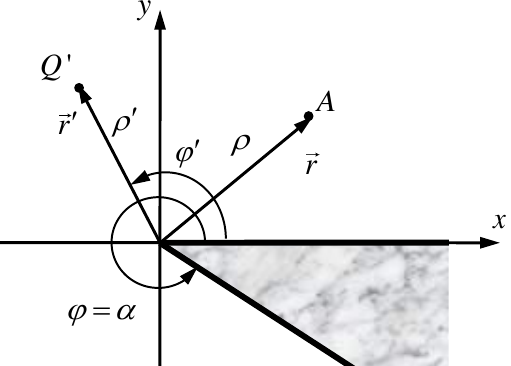
\includegraphics[width=.3\paperheight]{content/caem/pictures/conducting_wedge.png}
\end{center}
\begin{enumerate}
  \item Formulation in cylindrical coordinates:
        \begin{align*}
          &\dfrac{1}{\rho} \dfrac{\partial}{\partial\rho}\left(\rho \dfrac{\partial}{\partial\rho}G\right)
          + \dfrac{1}{\rho^{2}}\dfrac{\partial^{2}}{\partial \varphi^{2}}G\\
          = &-\dfrac{1}{\rho} \delta(\rho - \rho') \delta(\varphi - \varphi')
        \end{align*}
  \item Seperation ansatz for homogeneous problem:
        \begin{align*}
          &\phi(\rho, \varphi) = h(\rho) f(\varphi),\\
          &\underbrace{\dfrac{\rho}{h(\rho)} \dfrac{\partial}{\partial\rho} \left[\rho \dfrac{\partial}{\partial\rho} h(\rho)\right]}_{\nu^{2}}
            + \underbrace{\dfrac{1}{f(\varphi)} \dfrac{\partial^{2}}{\partial\varphi^{2}} f(\varphi)}_{-\nu^{2}}
            = 0\\
          & \dfrac{\partial^{2}}{\partial\varphi^{2}}f(\varphi) + \nu^{2}f(\varphi) = 0
            \implies f(\varphi) \text{\texttildelow} \left\{e^{\pm j\nu \varphi}\right\}
          \begin{Bmatrix} \sin(\nu\varphi)\\ \cos(\nu\varphi) \end{Bmatrix}\\
          & \dfrac{\partial}{\partial\rho} \left[\rho \dfrac{\partial}{\partial\rho} h(\rho)\right] - \nu^{2}\dfrac{h(\rho)}{\rho} = 0
            \implies h(\rho) \, \text{\texttildelow} \, \rho^{\nu}, \rho^{-\nu}
        \end{align*}
  \item Ansatz for $G_{D}$ (fulfills BC in $\varphi$ and symmetry in $\varphi, \varphi'$)
        \begin{equation*}
          G_{D}(\rho, \varphi, \rho', \varphi') = \sum\limits_{n=1}^{\infty} g_{n}(\rho, \rho')
          \dfrac{2}{\alpha}
          \sin\left(\dfrac{n\pi}{\alpha} \varphi\right)
          \sin\left(\dfrac{n\pi}{\alpha} \varphi'\right)
        \end{equation*}
  \item Solution after reducing problem to 1D and solving coefficients using the ``jump'' equation:
        \begin{align*}
          &G_{D}(\rho, \varphi, \rho', \varphi')\\
          = &\dfrac{1}\pi \sum\limits_{n=1}^{\infty} \dfrac{1}{n}
          \sin\left(\dfrac{n\pi}{\alpha} \varphi\right)
          \sin\left(\dfrac{n\pi}{\alpha} \varphi'\right)
          \rho_{<}^{\frac{n\pi}{\alpha}}
          \rho_{>}^{-\frac{n\pi}{\alpha}}
        \end{align*}
\end{enumerate}

\subsection{Linearly Independant Solutions of the Laplace Equation in Spherical Coordinates}
\begin{align*}
  &\Delta\phi(r,\vartheta, \varphi) = 0\\
  &\dfrac{1}{r^{2}}\dfrac{\partial}{\partial r}\left(r^{2} \dfrac{\partial}{\partial r} \phi(\cdot)\right)\\
  + &\dfrac{1}{r^{2}\sin\vartheta} \dfrac{\partial}{\partial\vartheta} \left(\sin\vartheta \dfrac{\partial}{\partial\vartheta} \phi(\cdot)\right)\\
  + &\dfrac{1}{r^{2}\sin^{2}\vartheta} \phi(\cdot) = 0
\end{align*}
\begin{itemize}
        \item Solution by seperation ansatz
        \begin{equation*}
          \phi(r,\vartheta,\varphi) = U(r)Y(\vartheta, \varphi),
        \end{equation*}
        \begin{align*}
          &\underbrace{\dfrac{1}{U(r)} \dfrac{\partial}{\partial r} \left(r^{2} \dfrac{\partial}{\partial r} U(r)\right)}_{n(n+1)}\\
          + &\dfrac{1}{Y(\vartheta,\varphi)} \left[ \dfrac{1}{\sin\vartheta} \dfrac{\partial}{\partial\vartheta} \left(\sin\vartheta \dfrac{\partial}{\partial\vartheta} Y(\vartheta, \varphi)\right)\right.\\
          &\left.+ \dfrac{1}{\sin^{2}\vartheta} \dfrac{\partial^{2}}{\partial\varphi^{2}} Y(\vartheta, \varphi) \right] = 0
        \end{align*}
  \item Solutions to the homogeneous problems:
        \begin{align*}
          &U(r) \,\text{\texttildelow}\, \begin{cases}r^{n},\\ r^{-(n+1)},\end{cases}\\
          &Y(\vartheta,\varphi) \,\text{\texttildelow}\, Y_{n,m}(\vartheta,\varphi)\text{ (sphere harmonics)}\\
        \end{align*}
\end{itemize}
\begin{info}{(Associated) Legendre Polynomials}
  Given the associated Legendre DE
  \begin{align*}
    &\dfrac{1}{\sin\vartheta}\dfrac{\mathrm{d}}{\mathrm{d}\vartheta}
    \left(\sin\vartheta \dfrac{\mathrm{d}}{\mathrm{d}\vartheta}V(\vartheta)\right)\\
    + &\left[\nu(\nu+1) - \dfrac{m^{2}}{\sin^{2}\vartheta}\right] V(\vartheta) = 0,
  \end{align*}
  using a substitution $\cos\vartheta = x$ and a power series ansatz $V(x) = \sum\limits_{k=0}^{\infty}a_{k}x^{k}$ yields an orthogonal system of functions over $|x|\leq 1$ which solve the problem.\\
  They are known as the associated Legendre polynomials of 1st ($P_{n}^{m}(x)$) and 2nd ($Q_{n}^{m}(x)$) kind:
  \begin{align*}
    P_{n}^{m}(x) &= (-1)^{m}(1-x^{2})^{\frac{m}{2}} \dfrac{\mathrm{d}^{m}}{\mathrm{d}x^{m}} P_{n}(x)\\
    &= \dfrac{(-1)^{m}}{2^{n}n!} \left(1 - x^{2}\right)^{\frac{m}{2}}\dif{n+m}{}{x}(x^{2}-1)^{n},
  \end{align*}
  \begin{align*}
    &Q_{n}^{m}(x) = (-1)^{m}(1-x^{2})^{\frac{m}{2}} \dfrac{\mathrm{d}^{m}}{\mathrm{d}x^{m}} Q_{n}(x)\\
    &\text{n: degree of the function}\\
    &\text{m: order of the function}\\
    &-n \leq m \leq n
  \end{align*}
\end{info}
\begin{recipe}{Sphere harmonics $Y_{n,m}(\cdot)$}
  Given the DE:
  \begin{align*}
    &\dfrac{1}{\sin\vartheta}\dfrac{\mathrm{d}}{\mathrm{d}\vartheta}
    \left(\sin\vartheta \dfrac{\mathrm{d}}{\mathrm{d}\vartheta}Y_{n,m}(\vartheta)\right)\\
    + &\left[n(n+1) - \dfrac{1}{\sin^{2}\vartheta}\dfrac{\partial^{2}}{\partial\varphi^{2}}\right] Y_{n,m}(\vartheta, \varphi) = 0,
  \end{align*}
  the solution is given by the sphere harmonics functions:
  \begin{align*}
    Y_{m,n}(\vartheta,\varphi) = &\sqrt{\dfrac{(2n+1)(n-m)!}{4\pi(n+m)!}}\\
                           &\cdot (P_{n}^{m}(\cos\vartheta)\,e^{jm\varphi}),\\
  \end{align*}
  which build an orthogonal system of functions in $\{Y_{n,m}, Y_{n,m}^{*}\}$.
\end{recipe}

\subsection{Constructing of a Free-Space Green's Function in Spherical Coordinates}
\begin{enumerate}
  \item Express the Poisson equation in spherical coordinates.
  \item Using the seperation ansatz $G(r,\vartheta,\varphi) = U(r)Y(\vartheta,\varphi)$, solve the homogenous problems in order to fulfill the BC.
  \item Ansatz for $G(\cdot)$:
        \begin{equation*}
          G(\cdot) = \sum\limits_{n=0}^{\infty}\sum\limits_{m=-n}^{n}g_{n}(r,r') Y_{n,m}(\vartheta,\varphi) Y_{n,m}^{*}(\vartheta',\varphi')
        \end{equation*}
\end{enumerate}

\subsection{Constructing Green's functions in 2 or 3 dimensions by reducing to 1D problem}
\begin{enumerate}
  \item Express the problem $\mathcal{L}\{G(\bs{r}-\bs{r'})\} = -\delta(\bs{r}-\bs{r'})$ in an appropriate coordinate system for the boundary conditions.
        \begin{equation*}
          \mathcal{L}\left\{G(q_{1}, q_{2}, q_{3})\right\} = -\delta(q_{1}-q_{1}') \delta(q_{2}-q_{2}') \delta(q_{3}-q_{3}')
        \end{equation*}
  \item Find solutions to the homogeneous problems (eigenfunctions corresponding to operator):
        \begin{align*}
          \mathcal{\hat{L}} \left\{U(q_{1})\right\} = c_{1}U(q_{1}) & & U_{m}(q_{1})\\
          \mathcal{\tilde{L}} \left\{V(q_{2})\right\} = c_{2}V(q_{2}) & \implies & V_{n}(q_{2})\\
          \mathcal{\bar{L}} \left\{W(q_{3})\right\} = c_{3}W(q_{3}) & & W_{l}(q_{3})
        \end{align*}
  \item Reduce to new 1D problem using \textbf{completeness} (term by term equality) and \textbf{orthogonality} in one or two coordinates:
        \begin{align*}
          &G = \sum\limits_{n} g_{n}(q_{3},q'_{3}) U_{n}(q_{1},q_{2})U_{n}(q'_{1},q'_{2})\\
          &\sum\limits_{n} U_{n}(q_{1},q_{2}) U_{n}(q'_{1},q'_{2}) = \delta(q_{1}-q'_{1})\delta(q_{2}-q'_{2})\\
          &\implies \mathcal{L'}\left\{g_{n}(q_{3},q'_{3})\right\} = -\delta(q_{3}-q'_{3})
        \end{align*}
  \item Find 1D Green's function for the new 1D problem
        \begin{equation*}
          \mathcal{L'}\left\{g_{n}(q_{3},q'_{3})\right\} = -\delta(q_{3}-q'_{3})
        \end{equation*}
\end{enumerate}

\subsection{Systematic procedure for a Green's function of 2nd order ordinary differential operator}
\begin{equation*}
  \dfrac{\partial}{\partial x}\left(p(x) \dfrac{\partial}{\partial x} g(\cdot)\right) - q(x)g(\cdot) = -\delta(x-x')
\end{equation*}
\begin{itemize}
  \item Use two linearly independant solutions $f_1$ and $f_2$ of homogeneous problem \(\mathcal{L}\{f_{1/2}(x)\} = 0\)
  \item Generate particular solutions on both sides of the source location
        \begin{align*}
          u_{1}(x) = A_{1} f_{1}(x) + A_{2} f_{2}(x), \quad x < x'\\
          u_{1}(x) = B_{1} f_{1}(x) + B_{2} f_{2}(x), \quad x > x'\\
        \end{align*}
  \item Choose a Green's function of the form
        \begin{equation*}
          g(x, x') = h \, u_{1}(x_{<})u_{2}(x_{>})
        \end{equation*}
  \item Determine the constant h according to
        \begin{equation*}
          h = \dfrac{-1}{p(x) \cdot \mathcal{W}\{u_{1}(x), u_{2}(x)\}}
        \end{equation*}
        whereas $\mathcal{W}\{\cdot\}$ is the Wronski determinant (``Jump'' equation is automatically fulfilled). $\mathcal{W}\{\cdot\}$ can either be calculated or looked up in textbooks such as \textit{Handbook of Mathematics} by \textsc{Abramowitz and Stegun}.
\end{itemize}

\begin{definition}{Wronski Determinant}
  \begin{equation*}
    \mathcal{W}\{f_{1}, f_{2}\} = f_{1}\cdot f_{2}' - f_{1}'\cdot f_{2},
  \end{equation*}
  and for linear combinations we get:
  \begin{equation*}
    \mathcal{W}\{u_{1}, u_{2}\} = (A_{1}B_{2} - A_{2}B_{1}) \cdot \mathcal{W}\{f_{1}, f_{2}\},
  \end{equation*}
  \begin{align*}
    &u_{1}(x) = A_{1}f_{1}(x) + A_{2}f_{2}(x),\\
    &u_{2}(x) = B_{1}f_{1}(x) + B_{2}f_{2}(x).
  \end{align*}
\end{definition}

\subsection{Solution of the Laplace Equation in Cylindrical Coordinates}
\begin{align*}
  \dfrac{1}{\rho}\dfrac{\partial}{\partial \rho}\left(\rho\dfrac{\partial}{\partial \rho}\phi(\cdot)\right) + \dfrac{1}{\rho^{2}}\dfrac{\partial^{2}}{\partial \phi^{2}} \phi(\cdot) + \dfrac{\partial^{2}}{\partial z^{2}} \phi(\cdot) = 0
\end{align*}
\begin{itemize}
  \item
\end{itemize}
\begin{info}{Wronski determinants of Bessel (Hankel) functions}
  \begin{tabular}{>{$}l<{$}>{$}l<{$}}
    \mathcal{W}\{J_{\nu}, J_{-\nu}\} &= -\dfrac{2}{\pi x} \sin(\nu x)\\\\
    \mathcal{W}\{J_{\nu}, N_{\nu}\} &= \dfrac{2}{\pi x}\\\\
    \mathcal{W}\{H_{\nu}^{(1)}, H_{\nu}^{(2)}\} &= -\dfrac{4j}{\pi x}\\\\
    \mathcal{W}\{J_{\nu}, H_{\nu}^{(1),(2)}\} &= \pm \dfrac{2j}{\pi x}\\\\
    \mathcal{W}\{I_{\nu}, I_{-\nu}\} &= -\dfrac{2}{\pi x} \sin(\nu x)\\\\
    \mathcal{W}\{I_{\nu}, K_{\nu}\} &= -\dfrac{1}{x}\\\\
  \end{tabular}
\end{info}

		\section{Variational Calculus}
        \lipsum[6]
		\section{Integral Equation Solutions}
        \lipsum[7]
		\section{Vector Solutions of Maxwell's Equations}
        \lipsum[8]
	\end{multicols*}
\end{document}
